%%%%%%%%%%%%%%%%%%%%%%%%%%%%%%%%%%%%%%%%%%%%%%%%%%%%%%%%%%%%%%%%%%%%%%%%%%%%
% AGUtmpl.tex: this template file is for articles formatted with LaTeX2e,
% Modified March 2009
%
% This template includes commands and instructions
% given in the order necessary to produce a final output that will
% satisfy AGU requirements.
%
% PLEASE DO NOT USE YOUR OWN MACROS
%
% For more information on using the AGUTeX macro package,
% see agudocs.tex or agudocs.pdf
%
%%%%%%%%%%%%%%%%%%%%%%%%%%%%%%%%%%%%%%%%%%%%%%%%%%%%%%%%%%%%%%%%%%%%%%%%%%%%
%
% All questions should be e-mailed to author.help@agu.org.
%
%%%%%%%%%%%%%%%%%%%%%%%%%%%%%%%%%%%%%%%%%%%%%%%%%%%%%%%%%%%%%%%%%%%%%%%%%%%%
%
% Step 1: set the \documentclass
%
% The three options for article format are: two-column (default),
% draft, for initial article submission; and galley for narrow
% single columns.
%
% PLEASE USE THE DRAFT OPTION TO SUBMIT YOUR PAPERS
% The draft option produces double spaced output
%
% Choose the journal abbreviation for the journal you are
% submitting to:

% jgrga JOURNAL OF GEOPHYSICAL RESEARCH
% gbc   GLOBAL BIOCHEMICAL CYCLES
% grl   GEOPHYSICAL RESEARCH LETTERS
% pal   PALEOCEANOGRAPHY
% ras   RADIO SCIENCE
% rog   REVIEWS OF GEOPHYSICS
% tec   TECTONICS
% wrr   WATER RESOURCES RESEARCH
% gc    GEOCHEMISTRY, GEOPHYSICS, GEOSYSTEMS

% (If you are submitting to a journal other than jgrga,
% substitute the initials of the journal for "jgrga" below)

\documentclass[draft,grl]{AGUTeX}

%%%%%%%%%%%%%%%%%%%%%%%%%%%%%%%%%%%%%%%%%%%%%%%%%%%%%%%%%%
%%%% optional article formats author might want to use

% To produce a galley version:
% \documentclass[galley,jgrga]{AGUTeX}

% To produce a two columned version:
% \documentclass[jgrga]{AGUTeX}

%%%%%%%%%%%%%%%%%%%%%%%%%%%%%%%%%%%%%%%%%%%%%%%%%%%%%%%%%%%%%%%%%%%%%%%%%
% OPTIONAL:
% To print your article using PostScript fonts, uncomment this:
% \usepackage{agu-ps}
% You many need to edit the top of agu-ps to use the names of the PS
% fonts on your system.

%%%%%%%%%%%%%%%%%%%%%%%%%%%%%%%%%%%%%%%%%%%%%%%%%%%%%%%%%%%%%%%%%%%%%%%%%
% OPTIONAL:
% To Create numbered lines:

% If you don't already have lineno.sty, you can download it from
% http://www.ctan.org/tex-archive/macros/latex/contrib/ednotes/
% (or google lineno.sty ctan), available at TeX Archive Network (CTAN).
% Take care that you always use the latest version.

% To activate the commands, uncomment \usepackage{lineno}
% and \linenumbers*[1]command, below:

\usepackage{lineno}
\linenumbers*[1]

%%%%%%%%%%%%%%%%%%%%%%%%%%%%%%%%%%%%%%%%%%%%%%%%%%%%%%%%%%%%%%%%%%%%%%%%%
% Figures and Tables
%

% When submitting articles through the GEMS system:
% COMMENT OUT ANY COMMANDS THAT INCLUDE GRAPHICS.
% (See FIGURES section near the end of the file)


%  Figures and Tables should be placed at the end of the article,
%  after the references.
%
%  Uncomment the following command to include .eps files
%  (comment out this line for draft format):
\usepackage[dvips]{graphicx}
%
%    Uncomment the following command to allow illustrations to print
%    when using Draft:
\setkeys{Gin}{draft=false}
%
% Substitute one of the following for [dvips] above
% if you are using a different driver program and want to
% proof your illustrations on your machine:
%
% [xdvi], [dvipdf], [dvipsone], [dviwindo], [emtex], [dviwin],
% [pctexps],  [pctexwin],  [pctexhp],  [pctex32], [truetex], [tcidvi],
% [oztex], [textures]
%
% See how to enter figures and tables at the end of the article, after
% references.
%
%% ------------------------------------------------------------------------ %%
%
%  ENTER PREAMBLE
%
%% ------------------------------------------------------------------------ %%

% Author names in capital letters:
\authorrunninghead{DAWE AND AUSTIN}

% Shorter version of title entered in capital letters:
\titlerunninghead{INFLUENCE OF THE CLOUD SHELL}

% Author mailing address: please repeat this command for
% each author and alphabetize authors:

\authoraddr{Philip Austin,
Department of Earth and Ocean Sciences, University of
British Columbia, 6339 Stores Road, Vancouver, BC, V6T 1Z4, Canada.
(paustin@eos.ubc.ca)}

\authoraddr{Jordan T. Dawe,
Department of Earth and Ocean Sciences, University of
British Columbia, 6339 Stores Road, Vancouver, BC, V6T 1Z4, Canada.
(jdawe@eos.ubc.ca)}

\begin{document}

%% ------------------------------------------------------------------------ %%
%
%  TITLE
%
%% ------------------------------------------------------------------------ %%


\title{The influence of the moist cloud shell on conserved tracer measurements 
of entrainment and detrainment}
%

%% ------------------------------------------------------------------------ %%
%
%  AUTHORS AND AFFILIATIONS
%
%% ------------------------------------------------------------------------ %%


%Use \author{\altaffilmark{}} and \altaffiltext{}

% \altaffilmark will produce footnote;
% matching altaffiltext will appear at bottom of page.
% May use \\ to start a new line.

\authors{Jordan T. Dawe\altaffilmark{1} and Philip Austin\altaffilmark{1}}

\altaffiltext{1}{Department of Earth and Ocean Sciences, 
                      University of British Columbia, Vancouver, BC, Canada}

%% ------------------------------------------------------------------------ %%
%
%  ABSTRACT
%
%% ------------------------------------------------------------------------ %%

% >> Do NOT include any \begin...\end commands within
% >> the body of the abstract.

\begin{abstract}
Direct measurements of entrainment and detrainment rates from LES model 
cloud fields produce values twice as large as those produced from bulk 
conserved tracer budget calculations.  This discrepancy is a result of 
neglect of the influence of the moist cloud shell upon the conserved 
tracer tendencies.  Correcting the entrainment and detrainment values 
to account for the effect of the moist cloud shell corrects this 
over-estimate.  
\end{abstract}

%% ------------------------------------------------------------------------ %%
%
%  BEGIN ARTICLE
%
%% ------------------------------------------------------------------------ %%

% The body of the article must start with a \begin{article} command
%
% \end{article} must follow the references section, before the figures
%  and tables.

\begin{article}

%% ------------------------------------------------------------------------ %%
%
%  TEXT
%
%% ------------------------------------------------------------------------ %%

\section{Introduction}

Proper simulation of the subgridscale effect of cumulus clouds in GCMs 
requires understanding the rates at which air is entrained into and detrained 
from the clouds. Cloud entrainment and detrainment rates exert influences on 
profiles of cloud properties, the height of the cloud tops, the amount of heat 
and moisture the clouds transport upwards, and the heights at which the clouds 
deposit that heat and moisture.  They also have effects on the vertical 
transport of aerosols out of the boundary layer and the rate at which 
chemical reactions can occur in those aerosols 
\citep{Barahona2007,Anldrejczuk2008}. 

LES simulations are often used to study the dynamics of cloud entrainment and 
detrainment.  Entrainment and detrainment rates are typically calculated in 
these simulations by recording budgets of bulk conserved tracer variables, such 
as the total humidity or the liquid water moist static energy, and inferring 
the amount of fluid exchange between cloud and clear air that is needed to 
balance the rate at which that tracer is being vertically advected within the 
cloud field \citep{Siebesma1995}.

Alternatively, entrainment and detrainment could simply be calculated directly 
from the LES velocity and tracer fields.  \cite{Romps2010} recently presented 
a technique to directly measure entrainment and detrainment in this manner, 
and found that the direct measurement produced values twice as large as tracer 
budget calculations.  Romps attributed this difference to the assumption made 
in bulk tracer calculations that the fluid exchanged between clouds and 
environment had the mean properties of the cloud or environment, respectively.
Here we derive a correction to the direct mass flux due to the presence of 
the moist, negatively buoyant shell of evaporated cloud air that surrounds a 
cloud to make the direct flux compatible with bulk tracer calculations.

%==============================================================================

\section{Comparison of Siebesma and Romps bulk tracer calculations}

\cite{Siebesma1995} derive equations for entrainment and detrainment from a 
simple entraining cloud plume based on conserved bulk tracer properties:
\begin{equation}
  \label{eq:siebesma_entrainment}
    E_{\chi} = \frac{- M_c \frac{\partial \chi_c}{\partial z}
        - \frac{\partial \rho a \overline{w' \chi'}^c}{\partial z}
        - \rho a \frac{\partial \chi_c}{\partial t}
        + a \rho \left(\frac{\partial \bar{\chi}}{\partial t}\right)_{forcing}}
        {\chi_c - \chi_e}
\end{equation}
and
\begin{equation}
  \label{eq:siebesma_detrainment}
    D_{\chi} = \frac{- M_c \frac{\partial \chi_e}{\partial z}
        + \frac{\partial \rho (1 - a) \overline{w' \chi'}^e}{\partial z}
        + \rho (1-a) \frac{\partial \chi_e}{\partial t}
     - \rho (1-a) \left(\frac{\partial \bar{\chi}}{\partial t}\right)_{forcing}}
        {\chi_c - \chi_e}
\end{equation}
Here $\chi$ represents any conserved bulk tracer, such as total water ($q_t$, 
kg kg$^{-1}$) or liquid water moist static energy ($h$, J kg$^{-1}$); $a$ is 
the fractional cloud core area; $M_c$ is vertical cloud core mass flux 
(kg m$^{-2}$ s$^{-1}$); $w$ is vertical velocity (m s$^{-1}$); $e$ and $c$ 
sub- and super-scripts denote values conditionally sampled in the cloud 
environment and core; primed values represent anomalies relative to the 
horizontal mean; overbars represent horizontal averaging; and $E_{\chi}$ and 
$D_{\chi}$ are the bulk tracer entrainment into and detrainment out of the 
cloud plume in kg m$^{-3}$ s$^{-1}$.

\cite{Romps2010} derives alternate equations equivalent to 
(\ref{eq:siebesma_entrainment}) and (\ref{eq:siebesma_detrainment}) which use
direct tracer flux calculations in place of horizontally averaged tracer 
budgets.  \cite{Romps2010} derives tracer entrainment and detrainment to be:
\begin{equation}
  \label{eq:romps_entrainment}
  E_{\chi} = \frac{\chi_{c}(E_d-D_d) - (\overline{e\chi} - \overline{d\chi})}{(\chi_{c} - \chi_{e})}
\end{equation}
\begin{equation}
  \label{eq:romps_detrainment}
  D_{\chi} = \frac{\chi_{e}(E_d-D_d) - (\overline{e\chi} - \overline{d\chi})}{(\chi_{c} - \chi_{e})}
\end{equation}
where E - D is calculated directly from model mass fluxes through the relation
\begin{equation}
  \label{eq:romps_e_minus_d}
  e - d = \frac{\partial}{\partial t}(A\rho) + \nabla \cdot (\rho u A) 
\end{equation}
and $e\chi - d\chi$ is 
\begin{equation}
  \label{eq:romps_e_minus_d}
  e\chi - d\chi = \frac{\partial}{\partial t}(\chi A \rho) + \nabla \cdot (\chi \rho u A) 
\end{equation}
Here, A is blah, e is blah, $E_d$ and $D_d$ are blah, u is blah

Using these two derivations of $E_{\chi}$ and $D_{\chi}$ we can compare the 
error introduced by the numerical scheme used to calculate these values.

We have implemented the direct entrainment calculation scheme of 
\cite{Romps2010} in the System for Atmospheric Modelling 
\citep[SAM;][]{Khairoutdinov2003}, allowing the model to calculate average 
cloud core entrainment and detrainment over fifteen minute periods.  We have 
run this schemes in a standard GCSS Barbados Oceanographic and Meteorological 
Experiment (BOMEX) LES simulation \citep{Holland1973, Siebesma2003}.  
The model was run with a domain extent of 6.4 km x 6.4 km in the horizontal and 
3.2 km in the vertical at 25 metre grid resolution in all directions.  Model 
cloud area, vertical velocity, and cloud core entrainment diagnosed from bulk 
conserved tracer budgets agree well with the results presented in 
\cite{Siebesma2003}.  The model was run for 6 hours, and the first three hours 
of simulation were discarded as the model was still adjusting into 
steady-state.  15 minute averages were output for the terms of each of our 
calculations.

  We have performed this calculation for both $q_t$ and $h$, but the 
results are essentially identical and we will confine our discussion to the 
entrainment and detrainment inferred using $q_t$ as the conserved bulk tracer.  


%===================================================

\section{Correction of direct flux calculations}

Here we derive a correction to direct flux measurements of entrainment and 
detrainment to make them compatible with a simple entrainment plume framework.



\subsection{Siebesma method}

Here we derive a correction to their equations (5.3a) and (5.3b) to account 
for the radial variation in cloud properties.  We start our derivation by 
modifying equation (5.1) from \cite{Siebesma1995}, replacing the mean cloud 
core and environment values of the bulk tracers in the entrainment and 
detrainment terms with the cloud and environment values at the cloud surface:
\begin{eqnarray}
  \label{eq:entrainment_derivation_1}
    \rho \frac{\partial a \chi_c}{\partial t} 
    = - \frac{\partial M_c \chi_c}{\partial z} 
    + E \chi_{se} - D \chi_{sc} 
    - \frac{\partial \rho a \overline{w' \chi'}^c}{\partial z} 
    + a \rho \left(\frac{\partial \bar{\chi}}{\partial t}\right)_{forcing}
\end{eqnarray}
\begin{eqnarray}
  \label{eq:detrainment_derivation_1}
    \rho \frac{\partial (1 - a) \chi_e}{\partial t}
    = \frac{\partial M_c \chi_e}{\partial z} 
    - E \chi_{se} + D \chi_{sc} 
    - \frac{\partial \rho (1 - a) \overline{w' \chi'}^e}{\partial z} 
    + \rho (1 - a) \left(\frac{\partial \bar{\chi}}{\partial t}\right)_{forcing}
\end{eqnarray}

To solve these equations we make use of the continuity equation for a cloud 
plume,
\begin{equation}
   \label{eq:continuity}
   \rho \frac{\partial a}{\partial t} + \frac{\partial M_c}{\partial z} = E - D
\end{equation}
This allows us to write:
\begin{eqnarray}
  \label{eq:entrainment_derivation_2}
    E (\chi_{se} - \chi_c) + D (\chi_c - \chi_{sc}) 
    = M_c \frac{\partial \chi_c}{\partial z}
    + \frac{\partial \rho a \overline{w' \chi'}^c}{\partial z} 
    + \rho a \frac{\partial \chi_c}{\partial t}
    - a \rho \left(\frac{\partial \bar{\chi}}{\partial t}\right)_{forcing}
\end{eqnarray}
\begin{eqnarray}
  \label{eq:detrainment_derivation_2}
    D (\chi_e - \chi_{sc}) + E (\chi_{se} - \chi_e)
    = M_c \frac{\partial \chi_e}{\partial z}
    - \frac{\partial \rho (1 - a) \overline{w' \chi'}^e}{\partial z} 
    - \rho (1 - a) \frac{\partial \chi_e}{\partial t}
    + \rho (1 - a) \left(\frac{\partial \bar{\chi}}{\partial t}\right)_{forcing}
\end{eqnarray}

Unlike the derivation in \cite{Siebesma1995}, this step does not complete our 
solution since the $(\chi_{se} - \chi_e)$ and $(\chi_c - \chi_{sc})$ terms 
no longer cancel.  Instead, the solution becomes:
\begin{equation}
  \label{eq:final_entrainment}
    E = \frac{(\chi_{sc} - \chi_e)E_0 + (\chi_c - \chi_{sc})D_0}
             {(\chi_{sc} - \chi_{se})}
\end{equation}
\begin{equation}
  \label{eq:final_detrainment}
    D = \frac{(\chi_{se} - \chi_e)E_0 + (\chi_c - \chi_{se})D_0}
             {(\chi_{sc} - \chi_{se})}
\end{equation}
where $E_0$ and $D_0$ represent the entrainment and detrainment values
calculated in \cite{Siebesma1995}:
\begin{equation}
  \label{eq:E_0_equation}
    E_0 = \frac{- M_c \frac{\partial \chi_c}{\partial z}
        - \frac{\partial \rho a \overline{w' \chi'}^c}{\partial z}
        - \rho a \frac{\partial \chi_c}{\partial t}
        + a \rho \left(\frac{\partial \bar{\chi}}{\partial t}\right)_{forcing}}
        {\chi_c - \chi_e}
\end{equation}
and
\begin{equation}
  \label{eq:D_0_equation}
    D_0 = \frac{- M_c \frac{\partial \chi_e}{\partial z}
        + \frac{\partial \rho (1 - a) \overline{w' \chi'}^e}{\partial z}
        + \rho (1-a) \frac{\partial \chi_e}{\partial t}
     - \rho (1-a) \left(\frac{\partial \bar{\chi}}{\partial t}\right)_{forcing}}
        {\chi_c - \chi_e}
\end{equation}

Finally, we can invert equations (\ref{eq:final_entrainment}) and 
(\ref{eq:final_detrainment}) to use the direct values of \cite{Romps2010} to 
calculate equivalent tracer entrainment values:
\begin{equation}
  \label{eq:inverted_entrainment}
    E_0 = \frac{(\chi_{c} - \chi_{se})E - (\chi_{c} - \chi_{sc})D}
             {(\chi_{c} - \chi_{e})}
\end{equation}
\begin{equation}
  \label{eq:inverted_detrainment}
    D_0 = \frac{(\chi_{sc} - \chi_{e})D - (\chi_{se} - \chi_{e})E}
             {(\chi_{c} - \chi_{e})}
\end{equation}

We can immediately see this correction has two effects.  First, it reduces
the direct entrainment by a factor of
$(\chi_{c} - \chi_{se})/(\chi_{c} - \chi_{e})$ and the direct detrainment 
by a factor of $(\chi_{sc} - \chi_{e})/(\chi_{c} - \chi_{e})$, to account for 
the greater quantity of edge and shell air needed to balance the bulk tracer 
tendency terms.  Second, the correction also adds a term to represent the 
changes in the mean core and environment properties due to entraining parcels 
moister than the environmental mean and detraining parcels dryer than the cloud 
mean.  Note that this correction does not alter the value of $E-D$, as can be 
easily confirmed by subtracting equation (\ref{eq:final_detrainment}) from 
equation (\ref{eq:final_entrainment}).



%==============================================================================

These equations assume that fluid entraining into the cloud has the mean 
properties of the cloud core environment is incorrect.  The errors induced by 
this assumption can immediately be seen in the large negative bulk tracer 
detrainment values near cloud base (Figure \ref{fig:direct_vs_tracer}b).  
These negative values occur because entrainment at cloud base is due to 
thermodynamic changes instead of mechanical mixing.  Only the moistest 
environmental parcels condense at cloud base to form clouds, and this means 
that fluid entrained at cloud base is moister than the mean environment.  As 
this moist condensing fluid essentially has the same properties as cloud base 
air it does not drive changes in the mean cloud properties, and thus does not 
appear as entrainment in equation (\ref{eq:siebesma_entrainment}).  However, the 
removal of the moistest fluid from the environment does result in drying of 
the environmental mean, and this drying is interpreted as negative 
detrainment by equation (\ref{eq:siebesma_detrainment}).



%-----------------------------------------------------------------------------


To calculate values for $E$ and $D$ from the tracer budgets, we evaluate the 
terms on the right hand side of equations (\ref{eq:siebesma_entrainment}) and 
(\ref{eq:siebesma_detrainment}) directly in the model code and output 15 minute averages 
of the calculated values.  Comparison of the direct entrainment scheme with the 
bulk tracer method confirms the direct scheme of \cite{Romps2010} measures 
entrainment values approximately 2 times larger than the bulk tracer method.

%-----------------------------------------------------------------------------

\section{Radial cloud structure}

The bulk tracer calculations have one obvious source of bias: the assumption 
that all fluid entrained or detrained from the cloud has the mean properties of 
the environment or cloud, respectively.  

Examination of the cloud core edge properties (cloud core model grid cells 
that are horizontally adjacent to non-core cells) shows the cloud core edge has 
nearly the same properties as the mean core, while the cloud core shell 
properties (non-core cells that are horizontally adjacent to core cells) 
are significantly different than mean environment properties (Figure 
\ref{fig:shell_edge_profiles}).  This is in agreement with previous results 
from both LES modelling and observations /citep{Heus2008}.





Applying these corrections to the tracer calculations of entrainment and 
detrainment roughly doubles the calculated values and results in much better 
agreement with our direct flux calculations (Figure 
\ref{fig:corrected_entrainment}).



1. Derive equations relating tracer and direct E/D
  Seibesma conversion
  Romps conversion
	Figure 1: siebesma vs romps error
  10% differences between seibesma and Romps calculation methods

2. Column profiles showing how large each tracer value is
    Figure 2: tracer profiles
    Shell values not the same as 'effective' values due to reynolds correlations
    calculate mean $qt_se$ and $qt_sd$ to compare with spatial shell

3. Compare conversion factors
    Figure 3: correction using simply shell values, reynolds values

4. Eqt decomposition showing reynolds correlation magnitude
    relative error introduced by reynolds correlations


%==============================================================================

\section{Discussion and Conclusion}

Conclusions
Seibesma underestimates 'tracer' e/d by 10\% due to w interp, derivatives
Conversion between mass e/d and tracer e/d requires knowledge of cloud shell

The entrainment or detrainment value one considers to be correct will depend on 
the purpose for which they are used.  The correction to the bulk tracer 
calculation due to the cloud shell has little bearing on the entrainment and 
detrainment values needed for calculating cloud moisture and energy in GCM 
parameterizations, which only have access to large-scale mean bulk tracer 
values.  However, this correction may be important for calculating 
fluxes of properties that have different radial dependencies than $q_t$ or $h$, 
such as vertical momentum, which is negative in the shell \citep{Heus2008}, or 
for aerosols whose chemical properties are altered by reactions in the presence 
of liquid water \citep{Hoppel1994}.  In any case, the agreement between our 
direct flux method and the bulk tracer method corrected for the influence of 
the cloud shell suggests the shell correction removes a significant bias when 
estimating the total mass exchange between clouds and environment.

The bulk tracer calculations given by \cite{Siebesma1995} calculate the amount
of fluid with the mean properties of cloud and environment that would need to
be exchanged to balance advection and thermodynamic changes, not the true mass
fluxes that occur between cloud and environment.  To calculate the actual mass
fluxes the bulk tracer equations must at least be corrected for the effect of
the moist shell of evaporated air around the cloud.  This correction increases
entrainment and detrainment rates by a factor of 2-3.  This suggests that the
presence of the moist cloud shell has a significant role in mediating fluxes
between the clouds and the environment, and may be an important factor in 
improving parameterizations of shallow convection.


%%% End of body of article:

%%%%%%%%%%%%%%%%%%%%%%%%%%%%%%%%
%% Optional Appendix goes here
%
%%%%%%%%%%%%%%%%%
% Geophysical Research Letters only allows an appendix without a letter.
%% You can get this result with
%  \section*{Appendix}
%  or
%  \section*{Appendix: Title}
%%%%%%%%%%%%%%%%%
%
% \appendix resets counters and redefines section heads
% but doesn't print anything.
% After typing  \appendix
%
% \section{Here Is Appendix Title}
% will print
% Appendix A: Here Is Appendix Title
%
% \section*{Appendix}
% will print
% Appendix
%
% \section*{Appendix: Here Is Appendix Title}
% will print
% Appendix: Here Is Appendix Title
%
% For only 1 appendix \appendix \section{Appendix} is preferred.
% which will print
% Appendix A

%%%%%%%%%%%%%%%%%%%%%%%%%%%%%%%%%%%%%%%%%%%%%%%%%%%%%%%%%%%%%%%%
%
% Optional Glossary or Notation section, goes here
%
%%%%%%%%%%%%%%
% Glossary only allowed in Reviews of Geophysics
% \section*{Glossary}
% \paragraph{Term}
% Term Definition here
%
%%%%%%%%%%%%%%
% Notation -- End each entry with a period.
% \begin{notation}
% Term & definition.\\
% Second Term & second definition.
% \end{notation}
%%%%%%%%%%%%%%%%%%%%%%%%%%%%%%%%%%%%%%%%%%%%%%%%%%%%%%%%%%%%%%%%
%
%  ACKNOWLEDGMENTS

\begin{acknowledgments}
Support for this work was provided by the Canadian Foundation for Climate and 
Atmospheric Science through the Cloud Aerosol Feedback and Climate network.
All figures were generated using the matplotlib library in the Python
programming language.
\end{acknowledgments}

%% ------------------------------------------------------------------------ %%
%
%  REFERENCE LIST AND TEXT CITATIONS
%
% Either type in your references using
% \begin{thebibliography}{}
% \bibitem{}
% Text
% \end{thebibliography}
%
% Or,
%
% If you use BiBTeX for your References, please produce your .bbl
% file and copy the contents into your paper here.
%
% Follow these steps:
% 1. Run LaTeX on your LaTeX file.
%
% 2. Run BiBTeX on your LaTeX file.
%
% 3. Open the new .bbl file containing the reference list and
%   copy all the contents into your LaTeX file here.
%
% 4. Comment out the old \bibliographystyle and \bibliography commands.
%
% 5. Run LaTeX on your new file before submitting.
%
% AGU does not want a .bib or a .bbl file, but asks that you
% copy in the contents of your .bbl file here.


%\begin{thebibliography}{}

\bibliography{shell_correction}
\bibliographystyle{agu}

%\bibitem[{\textit{Kilby}(2008)}]{jskilby}
%Kilby, J. S. (2008), Invention of the integrated circuit, {\it IEEE
%Trans. Electron Devices,} \textit{23}, 648--650.

%\bibitem[{\textit{Kilby et al.}(2008)}]{jskilbye}
%Kilby, J. S., S. Smith, and R. Jones (2008), Invention of the
%integrated circuit, {\it IEEE Trans. Electron Devices,} \textit{23},
%648--650.

%\end{thebibliography}

%Reference citation examples:

%...as shown by \textit{Kilby} [2008].
%...has been shown [\textit{Kilby et al.}, 2008].

%...as shown by \cite{jskilby}.
%...has been shown \citep{jskilbye}.


%% ------------------------------------------------------------------------ %%
%
%  END ARTICLE
%
%% ------------------------------------------------------------------------ %%

\end{article}

%% Enter Figures and Tables here:

% When submitting articles through the GEMS system:
% COMMENT OUT ANY COMMANDS THAT INCLUDE GRAPHICS.

% Figure captions go below this illustration; Table captions go above tables

\begin{figure}
  \label{fig:resolution_dependence}
  \noindent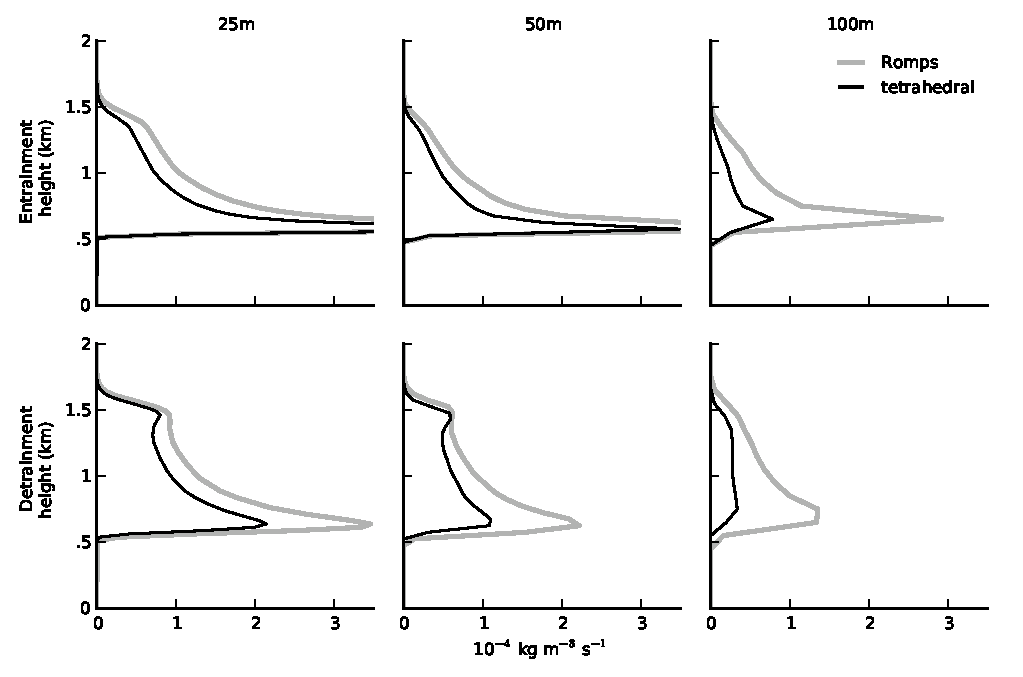
\includegraphics[width=20pc]{./figures/resolution_dependence}
  \caption{Mean profiles of a) Entrainment and b) Detrainment.}
\end{figure}

\begin{figure}
  \label{fig:shell_edge_profiles}
  \noindent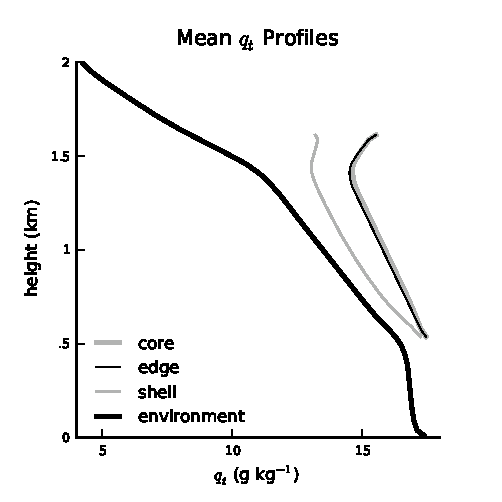
\includegraphics[width=29pc]{./figures/shell_edge_profiles_core}
  \caption{Mean profiles of $q_t$ in the cloud core (thick grey line), core 
edge (thin black line), core shell (thin grey line), and environment (thick 
black line).}
\end{figure}

\begin{figure}
  \label{fig:corrected_entrainment}
  \noindent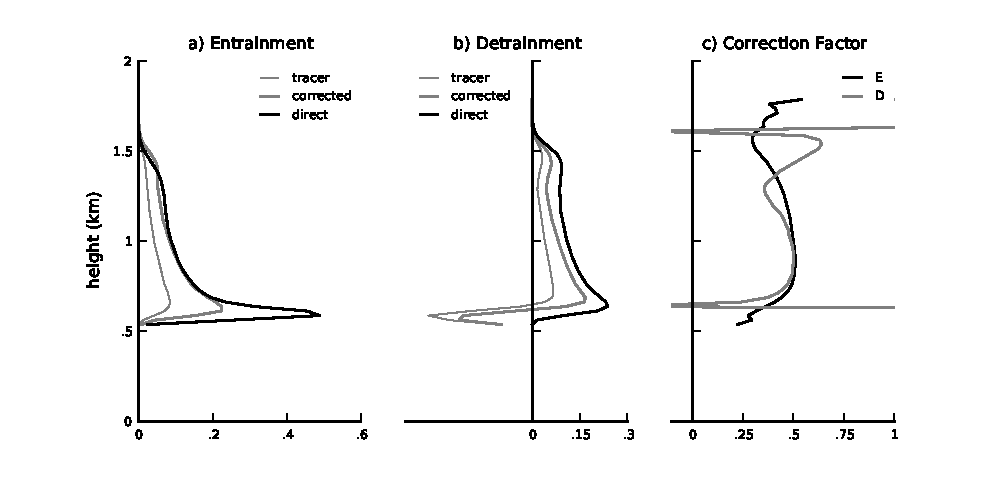
\includegraphics[width=39pc]{./figures/corrected_entrainment_core}
  \caption{Comparison of mean a) entrainment and b) detrainment profiles 
calculated using uncorrected bulk tracer budgets (thin grey line), bulk tracer 
budgets corrected for the presence of a moist cloud shell (thick grey line), and
direct flux calculations with tetrahedral surface interpolation (black line).
c) Ratio of corrected bulk tracer rates to the direct flux using
tetrahedral interpolation rates of entrainment (black) and detrainment (grey).
d) and e) are the same as a) and b) but for the fractional entrainment and
detrainment rates.}
\end{figure}

% ONE-COLUMN figure/table, including eps graphics
%
% \begin{figure}
% \noindent\includegraphics[width=20pc]{samplefigure.eps}
% \caption{Caption text here}
% \end{figure}
% \end{document}
%
% \begin{table}
% \caption{}
% \end{table}
%
% ---------------
% TWO-COLUMN figure/table
%
% \begin{figure*}
% \noindent\includegraphics[width=39pc]{samplefigure.eps}
% \caption{Caption text here}
% \end{figure*}
%
% \begin{table*}
% \caption{Caption text here}
% \end{table*}
%
% see below for how to make landscape figures or tables

%%% End the article here:

\end{document}

%%%%%%%%%%%%%%%%%%%%%%%%%%%%%%%%%%%%%%%%%%%%%%%%%%%%%%%%%%%%%%%


%% ------------------------------------------------------------------------ %%
%
%  IN-TEXT LISTS
%
%% ------------------------------------------------------------------------ %%

% Do not use bulleted lists; enumerated lists are okay.
% \begin{enumerate}
% \item
% \item
% \item
% \end{enumerate}

%% ------------------------------------------------------------------------ %%
%
%  EQUATIONS
%
%% ------------------------------------------------------------------------ %%

% Single-line equations are centered.

% Math coded inside display math mode \[ ...\]
% will not be numbered e.g.:
% \[ x^2=y^2 + z^2\]

% Math coded inside \begin{equation} and \end{equation} will
% be automatically numbered e.g.:
% \begin{equation}
% x^2=y^2 + z^2
% \end{equation}

% IF YOU HAVE MULTI-LINE EQUATIONS, PLEASE
% BREAK THE EQUATIONS INTO TWO OR MORE LINES
% OF SINGLE COLUMN WIDTH (20 pc, 8.3 cm)
% using double backslashes (\\).

% To create multiline equations, use the
% \begin{eqnarray} and \end{eqnarray} environment
% as demonstrated below.
\begin{eqnarray}
  x_{1} & = & (x - x_{0}) \cos \Theta \nonumber \\
        && + (y - y_{0}) \sin \Theta  \nonumber \\
  y_{1} & = & -(x - x_{0}) \sin \Theta \nonumber \\
        && + (y - y_{0}) \cos \Theta.
\end{eqnarray}

If you don't want an equation number, use the star form:
\begin{eqnarray*}...\end{eqnarray*}

% Break each line at a sign of operation
% (+, -, etc.) if possible, with the sign of operation
% on the new line.

% Indent second and subsequent lines to align with
% the first character following the equal sign on the
% first line.

% Use an \hspace{} command to insert horizontal space
% into your equation if necessary. Place an appropriate
% unit of measure between the curly braces, e.g.
% \hspace{1in}; you may have to experiment to achieve
% the correct amount of space.

% There is another multiline equation environment:
% \begin{aguleftmath}...\end{aguleftmath}
% The equation is aligned left and the second line indents to
% the width of a paragraph indent (AGU style)


%% ------------------------------------------------------------------------ %%
%
%  EQUATION NUMBERING: COUNTER
%
%% ------------------------------------------------------------------------ %%

% You may change equation numbering by resetting
% the equation counter or by explicitly numbering
% an equation.

% To explicitly number an equation, type \eqnum{}
% (with the desired number between the brackets)
% after the \begin{equation} or \begin{eqnarray}
% command.  The \eqnum{} command will affect only
% the equation it appears with; LaTeX will number
% any equations appearing later in the manuscript
% according to the equation counter.
%
% To reset the equation counter, place the setcounter{equation}
% command in front of your equation(s).
%\setcounter{equation}{0}

% Set the equation counter to 0 if the next
% number needed is 1 or set it to 7 if the
% next number needed is 8, etc.
%
% The \setcounter{equation} command does affect
% equations appearing later in the manuscript.

% If you have a multiline equation that needs only
% one equation number, use a \nonumber command in
% front of the double backslashes (\\) as shown in
% the multiline equation above.



%%%%%%%%%%%%%%%%%%%%%%%%%%%%%%%%%%%%%%%%%%%%%%%%%%%%%%
%% Landscape figure and table examples
%
% ---------------
% Landscape (broadside) figure/table
% (These objects will not display properly in draft mode, use galley.)
%
% ONE-COLUMN landscape figure and table
%
% \begin{landscapefigure}
% \includegraphics[height=.75\mycolumnwidth,width=42pc]{samplefigure.eps}
% \caption{Caption text here}
% \end{landscapefigure}
%
% \begin{landscapetable}
% \caption{Caption text here}
% \begin{tabular*}{\hsize}{@{\extracolsep{\fill}}lcccc}
% \tableline
% ....
% \tableline\\
% \multicolumn5l{(a) Algorithms from Numerical Recipes}\\
% \end{tabular*}
% \tablenotetext{}{}
% \tablecomments{}
% \end{landscapetable}
%
% FULL-PAGE landscape figures and tables
%
% \begin{figure*}[p]
% \begin{landscapefigure*}
% illustration here
% \caption{caption here}
% \end{landscapefigure*}
% \end{figure*}
%
% \begin{table}[p]
% \begin{landscapetable*}
% \caption{}
% \begin{tabular*}{\textheight}{@{\extracolsep{\fill}}lccrrrcrrr}
% ....
% \end{tabular*}
% \begin{tablenotes}
% ...
% \end{tablenotes}
% \end{landscapetable*}
% \end{table}
%
